\subsection{Hipotesis}
\begin{itemize}
	\item Las podas de factibilidad y optimalidad en mejor caso tienen complejidad lineal.
	\item Hacer un sort de los elementos de mayor a menor, hace que las podas sean m\'as efectivas.
	\item Hacer un sort de los elementos de menor a mayor, hace que las podas empeoren y sean mas parecidas a fuerza bruta
	\item La poda de factibilidad empeora a medida que el valor de los elementos se acercan a 0, y mejora a medida que el valor de los elementos se acercan al valor objetivo
	\item Fuerza Bruta depende unicamente de la cantida de items
\end{itemize}
\subsection{Consideraciones para las experimentaciones}
\subsubsection{Generaci\'on de elementos}
\begin{itemize}
	\item Se usa la funcion sort de c++ (ordena los elementos en forma creciente)
	\item Los conjuntos fueron generados aleatoriamente, con la funci\'on rand de c++ (distribucion uniforme) para poder analizar en caso promedio que pasaba con cada algoritmo, en el rango entre [0..V].
	\item la cantidad de iteracione es igual a 50, pues se logro ver durante la experimentaci\'on que los algoritmos se estabilizaban.
	\item El rango para la suma fue [15000...80000], porque es limitada por Programacion Dinamica, la cual pide memoria de tamaño n*W y al ser W tan grande, hace que no se pueda seguir experimentando.
	\item El rango para la cantidad de elementos fue [5...35], porque al querer analizar el caso promedio se toma el promedio de 50 iteraciones y los algoritmos exponenciales tard\'an demasiado.
\end{itemize}
\subsubsection{Im\'agenes y Complejidades}
\begin{itemize}
	\item Para medir el tiempo se tomó el promedio 50 de iteraciones
	\item Para todos los algoritmos se grafica el tiempo en el eje Y (en ns), y la cantidad de elementos en el eje X
	\item Para todos los algoritmos se dan 2 gr\'aficos, el primero es como crece en funci\'on de la cantidad de elementos, luego el segundo algoritmo dividido por su complejidad te\'orica
	\item Todos los gr\'aficos con excepci\'on del \'ultimo fueron hecho con la suma objetivo igual a 500(el ultimo gr\'afico no, para poder mostrar como afecta el valor de la suma al algoritmo de Programaci\'on din\'amica)
\end{itemize}	
\subsection{Complejidades Te\'oricas en la practica}
\subsubsection{Fuerza Bruta}
Fuerza Bruta no es afectada por el sort de los elemento, y al aplicarle el logaritmo en base dos se logra ver que es lineal, lo cual es esperado pues es exponencial en la cantidad de elementos con base igual a 2.
\begin{center}
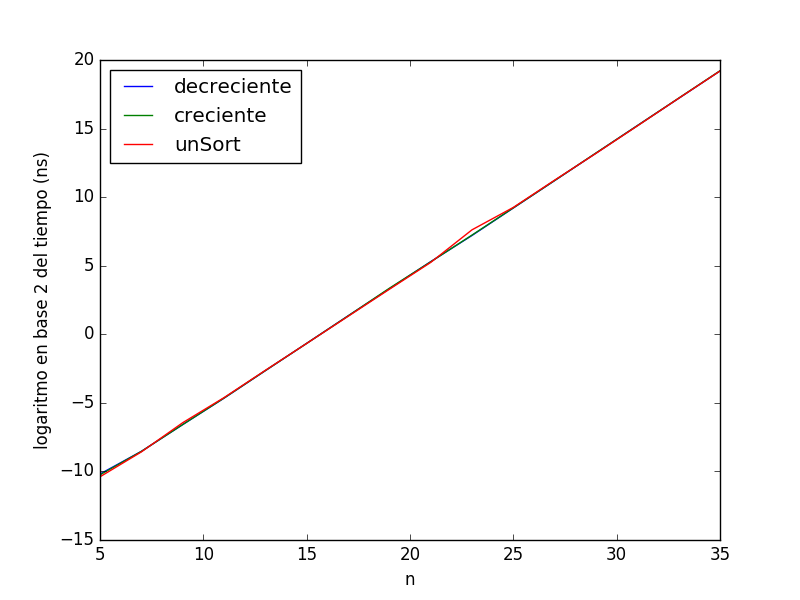
\includegraphics[width=16cm, height=11cm]{fbSort.png}
\end{center}

\subsubsection{Backtracking poda por factibilidad}
Tener los elementos ordenados de mayor a menor hace que la poda sea mas efectiva y empeora cuando el ordenamiento es de menor a mayor.\\
Se aplica logaritmo en base dos y se logra ver que el resultado es lineal.
\begin{center}
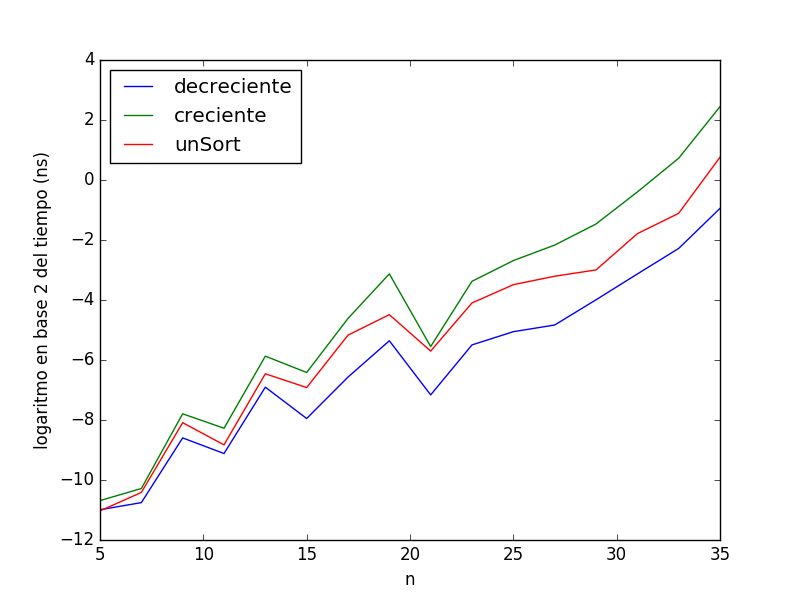
\includegraphics[width=16cm, height=11cm]{facSort.png}
\end{center}
\subsubsection{Backtracking poda por optimalidad}
El ordenamiento de los elementos afecta a la poda de optimalidad y se hace el mismo analisis que para la poda de factibilidad.
\begin{center}
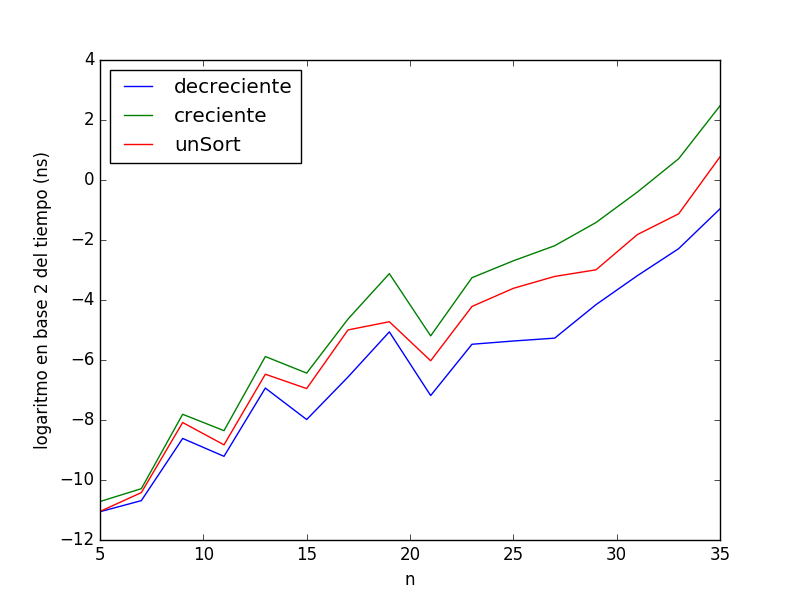
\includegraphics[width=16cm, height=11cm]{opSort.png}
\end{center}
\subsubsection{Programacion dinamica}
Para esta experimentacion se varia V y se compara el tiempo en funcion de el ordenamiento de los elementos.\\
El resultado es el esperado pues, en el grafico se ve como Programacion Dinamica es afectado directamente por el valor objetivo.
\begin{center}
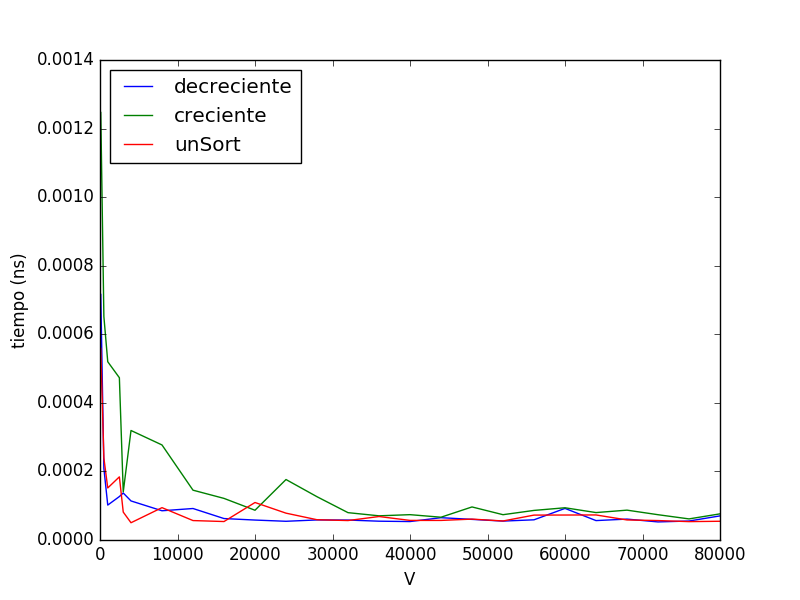
\includegraphics[width=16cm, height=11cm]{pdSuma.png}
\end{center}
%\begin{center}
%\includegraphics[width=16cm, height=11cm]{todosFac_objetivos_90000.png}
%\end{center}